\documentclass[12pt,a4paper,titlepage,headinclude,bibtotoc]{scrartcl}

%---- Allgemeine Layout Einstellungen ------------------------------------------

% Für Kopf und Fußzeilen, siehe auch KOMA-Skript Doku
\usepackage[komastyle]{scrpage2}
\pagestyle{plain}
\setheadsepline{0.5pt}[\color{black}]
\automark[section]{chapter}


%Einstellungen für Figuren- und Tabellenbeschriftungen
\setkomafont{captionlabel}{\sffamily\bfseries}
\setcapindent{0em}


%---- Weitere Pakete -----------------------------------------------------------
% Die Pakete sind alle in der TeX Live Distribution enthalten. Wichtige Adressen
% www.ctan.org, www.dante.de

% Sprachunterstützung
\usepackage[ngerman]{babel}

% Benutzung von Umlauten direkt im Text
% entweder "latin1" oder "utf8"
\usepackage[utf8]{inputenc}

% Pakete mit Mathesymbolen und zur Beseitigung von Schwächen der Mathe-Umgebung
\usepackage{latexsym,exscale,stmaryrd,amssymb,amsmath}


\usepackage[nointegrals]{wasysym}
\usepackage{eurosym}

% Anderes Literaturverzeichnisformat
%\usepackage[square,sort&compress]{natbib}
\usepackage{hyperref}
% Für Farbe
\usepackage{color}
\usepackage{graphicx}
\usepackage{wrapfig}
\usepackage{subfigure}

% Caption neben Abbildung
\usepackage{sidecap}

% Befehl für "Entspricht"-Zeichen
\newcommand{\corresponds}{\ensuremath{\mathrel{\widehat{=}}}}
% Befehl für Errorfunction
\newcommand{\erf}[1]{\text{ erf}\ensuremath{\left( #1 \right)}}

%Fußnoten zwingend auf diese Seite setzen
\interfootnotelinepenalty=1000

%Für chemische Formeln (von www.dante.de)
%% Anpassung an LaTeX(2e) von Bernd Raichle
%\makeatletter
%\DeclareRobustCommand{\chemical}[1]{%
  %{\(\m@th
  % \edef\resetfontdimens{\noexpand\)%
   %    \fontdimen16\textfont2=\the\fontdimen16\textfont2
    %   \fontdimen17\textfont2=\the\fontdimen17\textfont2\relax}%
 %  \fontdimen16\textfont2=2.7pt \fontdimen17\textfont2=2.7pt
  % \mathrm{#1}%
  % \resetfontdimens}}
%\makeatother

%Honecker-Kasten mit $$\shadowbox{$xxxx$}$$
\usepackage{fancybox}

%SI-Package
\usepackage{siunitx}

%keine Einrückung, wenn Latex doppelte Leerzeile
\parindent0pt

%Bibliography \bibliography{literatur} und \cite{gerthsen}
%\usepackage{cite}
\usepackage{babelbib}
\selectbiblanguage{ngerman}

\begin{document}

\begin{titlepage}
\centering
\textsc{\Large Praktikum zur Einführung in die physikalische Chemie,\\[1.5ex] Universität Göttingen}

\vspace*{1cm}

\rule{\textwidth}{1pt}\\[0.5cm]
{\huge \bfseries
  V6: Dissoziationskonstante\\[1.5ex]
  einer schwachen Säure}\\[0.5cm]
\rule{\textwidth}{1pt}

\vspace*{1cm}


\begin{Large}
\begin{tabular}{ll}
Durchführende: &  Alea Tokita, Julia Stachowiak\\
Assistentin: & Annemarie Kehl\\
 Versuchsdatum: & 18.01.2016\\
 Datum der 1. Abgabe: & 25.01.2016\\
 Datum der 2. Abgabe: & 04.02.16
\end{tabular}
\end{Large}

\vspace*{1cm}

\large
\begin{table} [h] 
\centering
\begin{tabular} {| p {3 cm}|| p {3 cm}|}
  \hline
  pH & $ K_{\mathrm{s}}$ \\\hline\hline
  $6,2$ & $ (14 \pm 5) \cdot 10^{-8}$\\
  $6,4$& $ (14 \pm 5) \cdot 10^{-8}$\\
  $6,6$& $ (13 \pm 5) \cdot 10^{-8}$\\
  $6,8$& $ (14 \pm 5) \cdot 10^{-8}$\\
  $7,0$& $ (9 \pm 5) \cdot 10^{-8}$\\
  $7,2$& $ (9 \pm 4) \cdot 10^{-8}$\\
  $7,4$& $ (9 \pm 5) \cdot 10^{-8}$\\
  $7,6$& $ (8 \pm 4) \cdot 10^{-8}$\\\hline
  &\\
  Auftragung& $ (15 \pm 5)\cdot 10^{-8}$ \\\hline\hline
  &\\
  Literaturwert (bei $22{~}^\circ$C) & $6,92 \cdot 10^{-8}$\\\hline
 \end{tabular}
\end{table}


\end{titlepage}

\tableofcontents

\newpage

\section{Theoretische Grundlagen}

Die Dissoziationskonstante der schwachen Säure p-Nitrophenol soll mittels Photometrie gemessen werden. \\
Dabei wird sich das Gleichgewicht der Säure in Wasser zunutze gemacht, da die dissoziierte und undissoziierte Form eine unterschiedliche Abschwächung der Lichtintensität aufweisen, welche mittels Photometrie bestimmt wird.\\

Säuren bilden in wässriger Lösung folgendes Gleichgewicht; $\mathrm{A^-}$ beschreibt den Säurerest.

\begin{equation}
\mathrm{HA}  \rightleftharpoons \mathrm{H^+} + \mathrm{A^-}
\end{equation}

Die Lage des Gleichgewichtes kann mithilfe des Massenwirkungsgesetzes beschrieben werden. Anstelle der Aktivitäten werden hier vereinfacht die Konzentrationen verwendet:\\

\begin{equation}
K_\mathrm{c} =\frac{c(\mathrm{H^+}) \cdot c\mathrm{(A^-)}}{c\mathrm{(HA)} \cdot c^0}
\end{equation}

$c^0$ beschreibt eine Konzentration von 1 $\mathrm{mol{~}l^{-1}}$, damit $K_\mathrm{S}$ einheitenlos wird. Um nicht mit hohen Potenzen zu rechnen, wird meist der negativ dekadische Logarithmus von $K_\mathrm{S}$ verwandt, um die Säurestärke anzugeben. Analog kann dies auch für Basen ("$pK_\mathrm{B}$") verwandt werden.\\

\begin{equation}
pK_\mathrm{S} = \mathrm{-log_{10}} \left(\frac{c(H^+)}{c^0}\right)
\end{equation}

Der $p$H-Wert ist folgendermaßen definiert:

\begin{equation}
p\mathrm{H}= \mathrm{-log}_{10}\left(\frac{c(H^+)}{c^0}\right)
\end{equation}

Anders als der Dissoziationsgrad gibt die Säurekonstante nicht das Verhältnis von dissoziierten Teilchen zur Einwaagekonzentration, sondern zu undissoziierten Teilchen im Gleichgewicht und ist daher eine $p$H-unabhängige aber temperaturabhängige Konstante.\\
Um $p$H-Werte auch bei Zugabe von Säure bzw. Base konstant zu halten, werden Pufferlösungen verwandt. Puffer sind schwache Säuren (oder Basen) mit ihrem konjugierten Salz. Bei Zugabe von Oxonium- bzw. Hydroxidionen werden diese durch den Puffer abgefangen.\\
Die geringe $p$H-Wert Änderung bei dieser Reaktion kann mittels der Henderson-Hasselbalch Gleichung beschrieben werden:\\

\begin{equation}
p\mathrm{H} = pK_\mathrm{S} + \mathrm{log}_\mathrm{10}\left(\frac{c\mathrm{(A^-)}}{c\mathrm{(HA)}}\right)
\end{equation}

In wässriger Lösung bildet p-Nitrophenol folgendes Gleichgewicht: 

\begin{figure} [h!]
\begin{center}
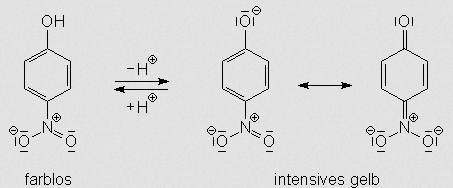
\includegraphics[scale=1]{Strukturformel2.png} \end{center}
\caption {Dissoziation und Lichtabsorption von p-Nitrophenol in wässriger Lösung\,\protect\footnotemark}
\end{figure}
\footnotetext{http://www.axel-schunk.de/experiment/edm0011n.gif.}


Eintreffende Strahlung kann von der dissoziierten Form im Gegensatz zu der undissoziierten Form durch Umklappen des freien Elektronenpaares absorbiert werden; somit ist die Abschwächung der Lichtintensität der dissoziierten Form größer.

\section{Experimentelles}
\subsection{Photometrie}
Die Verminderung der Lichtintensität $\mathrm{d}I$ der Lösung im Vergleich zu der Lichtintensität von Wasser $I_0$, ist ein Maß für die Konzentration der absorbierenden Substanz. Sie wird über den Weg $x$ genessen, hier gleichzusetzen mit der Küvettenschichtdicke $d$. Sie wird durch das Lambert-Beersche Gesetz beschrieben ergibt die Extinktion $E$:\\

\begin{equation}
E = \epsilon _{\lambda} \cdot c \cdot d = \mathrm{log_{10}}\left( \frac{I_0}{I}\right)
\end{equation}

$\epsilon_\mathrm{\lambda}$ beschreibt die Extinktionskonstante. 

Der Dissoziationsgrad $\alpha$ ist das Verhältnis aus der Konzentration von dissoziierten Teilchen im Vergleich zu der Einwaagekonzentration und damit auch das Verhältnis der gemessenen Extinktion $E_\mathrm{c}$ zu der Extinktion bei vollständiger Dissoziation $E_\infty$\\

\begin{equation}
\alpha = \frac{c(\mathrm{R^-})}{c_1} = \frac{E_\mathrm{c}}{E_\infty}
\end{equation}

Durch Einsetzen in das Ostwaldsche Verdünnungsgesetz und Umformung  ergibt sich die Säurekonstante:\\

\begin{equation}
K_\mathrm{S} =\frac{c( \mathrm{H} ^+) \cdot E_\mathrm{c}}{c^0 \cdot (E_\infty - E_\mathrm{c})}
\end{equation}

Zusätzlich kann $K_\mathrm{S}$ auch grafisch aus folgendem Zusammenhang bestimmt werden:\\

\begin{equation}
c(\mathrm{H}^+) = (\alpha^{-1} \cdot K_\mathrm{S} - K_\mathrm{S}) \cdot c^0
\end{equation}

Bei einer Auftagung von $c( \mathrm{H}^+)$ gegen $\alpha^{-1}$ ergibt sich $K_\mathrm{S}$ als Steigung:\\

\begin{equation}
\frac{d{~}c(\mathrm{H^+})}{d{~}\alpha^{-1}} = K_\mathrm{S}
\end{equation}

\subsection{Versuchsaufbau}

Folgende Grafik verdeutlicht die Funktionsweise des Photometers:

\begin{figure} [h!]
\begin{center}
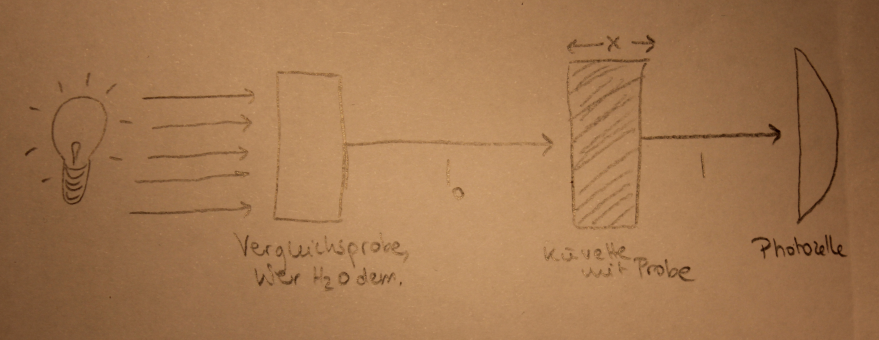
\includegraphics[scale=0.6]{Photometer.png} \end{center}
\caption {Funktionsweise eines Photometers}
\end{figure}

\subsection{Durchführung}
Die Extinktion wird bei 8 $p$H- Werten im Bereich von 6,2 bis 7,6 bei einer Wellenlänge von 420nm jeweils 6 mal im Verhältnis zu destilliertem Wasser gemessen.
Die Phosphat-Pufferlösungen für den jeweiligen $p$H-Wert werden aus einer 
$\frac{1}{15}\,\mathrm{mol{~}l^{-1}}\,\mathrm{KH_2PO_4}$\,-\,Lösung
 (Lösung A) und einer $\frac{1}{15}\,\mathrm{mol{~}l^{-1}}\,\mathrm{Na_2HPO_4}$-Lösung (Lösung B) hergestellt. 
 Dafür wird je ein vorgegebenes Volumen an Lösung B in einem Vollzylinder mit Lösung A auf 50 mL aufgefüllt. Anschließend werden 5 mL einer $1 \cdot 10^{-4}$ M p-Nitophenol-Lösung mit der hergestellten Pufferlösung in einem neuen Vollzylinder auf 50 mL aufgefüllt.\\
 
Außerdem werden 5 mL p-Nitrophenol mit 0,1 M NaOH auf 50 mL aufgefüllt, um die Extinktion bei vollständiger Dissoziation zu bestimmen. \\
 
Anschließend werden die Mittelwerte der Messungen gebildet und $\mathrm{c(H^+)}$ gegen $\alpha^-1$ aufgetragen. \\
Zusätzlich wird die Dissoziationskonstante errechnet.\\
 
Die Messung wird auf zwei Gruppen aufgeteilt, sodass jede Gruppe die Extinktion bei 4 $p$H-Werten misst.



\section{Auswertung}
Im Versuch wird die Messung der Extinktion für jeden $p$H, sowie für $E_{\infty}$, sechsmal durchgeführt. Anschließend wird daraus für jeden $p$H der Mittelwert der Extinktion gebildet. Es ergeben sich folgende Mittelwerte:

\begin{table} [h]
\begin{tabular} {| p {1,5 cm}|| p {3 cm}| p{2cm}|}
  \hline
  pH & $\overline{E}$& $E_{\infty}$ \\\hline\hline
  $6,2$& $0,182$&$0,988$\\
  $6,4$& $0,255$&$0,988$\\
  $6,6$& $0,347$&$0,988$\\
  $6,8$& $0,463$&$0,988$\\
  $7,0$& $0,659$&$1,378$\\
  $7,2$& $0,827$&$1,378$\\
  $7,4$& $0,948$&$1,378$\\
  $7,6$& $1,044$&$1,378$\\\hline
 

\end{tabular}
\end{table}

Nun lässt sich $K_{\mathrm{s}}$ folgendermaßen bestimmen:
\begin{align}
K_{\mathrm{s}} = \frac{c(\mathrm{H} _3 O^+) \cdot E_\infty}{c^{\circ} \cdot (E_\infty - E_{\mathrm{c}})} = \frac{10^{-p\mathrm{H}} \cdot E_\infty}{c^{\circ} \cdot (E_\infty - E_{\mathrm{c}})}
\end{align}

Ebenfalls kann nun $\alpha$ bestimmt werden durch:
\begin{align}
\alpha = \frac{E_{\mathrm{c}}}{E_{\infty}}
\end{align}


Somit ergibt sich:


\begin{table} [h]
\begin{tabular} {| p {1,5 cm}|| p {6 cm}| p{6cm}|}
  \hline
  $p$H & $K_{\mathrm{s}}$ & $\alpha$ \\\hline\hline
  &&\\
  $6,2$ & 
  $ K_{\mathrm{s}} = \frac{10^{-6,2} \cdot 0,988}{c^{\circ} \cdot (0,988 - 0,182) } = 14,25 \cdot 10^-8 
  $&
  $ \alpha = \dfrac{0,182}{0,988} = 0,184 $ 
  \\
  $6,4$& $13,85\cdot 10^{-8}$& $0,258$ \\
  $6,6$& $13,60\cdot 10^{-8}$& $0,351$\\
  $6,8$& $13,98\cdot 10^{-8}$& $0,468$\\
  $7,0$& $9,015\cdot 10^{-8}$& $0,478$\\
  $7,2$& $9,453\cdot 10^{-8}$& $0,600$\\
  $7,4$& $8,539\cdot 10^{-8}$& $0,788$\\
  $7,6$& $7,579\cdot 10^{-8}$& $0,757$\\\hline
 \end{tabular}
\end{table}

Des weiteren lässt sich $K_{\mathrm{s}}$ aus einer Auftragung bestimmen. Es gilt folgender Zusammenhang, aus welchem sich $K_{\mathrm{s}}$ als Steigung ergibt:
\begin{align}
c(\mathrm{H} ^+) = (\alpha^{-1} \cdot K_{\mathrm{s}} - K_{\mathrm{s}} ) \cdot c^{\circ} 
\end{align} 

Es muss also $c(\mathrm{H} ^+)$ gegen $\alpha^{-1}$ aufgetragen werden. Somit ergeben sich für die Auftragung folgende Werte:\\

\begin{table} [h!]
\begin{tabular} {| p {7 cm}| p {7 cm}|}
  \hline
  $c(\mathrm{H} ^+){~} \mathrm{in} {~}[\mathrm{mol \cdot l^-1}]$ & $\alpha^{-1}$ \\\hline\hline
  &\\
  $c(\mathrm{H} ^+) = 10^{-p\mathrm{H}} = 10^{-6,2} = 63 \cdot 10^{-8}$ & 
  $\alpha^{-1} = \frac{E_{\mathrm{c}}}{E_{\infty}} = \frac{0,182}{0,988} = 5,43$
  \\
  $40 \cdot 10^{-8}$ & $3,88$ \\
  $25\cdot 10^{-8}$& $2,85$\\
  $16\cdot 10^{-8}$& $2,13$\\
  $10\cdot 10^{-8}$& $2,09$\\
  $6,3\cdot 10^{-8}$& $1,67$\\
  $3,4\cdot 10^{-8}$& $1,45$\\
  $2,5\cdot 10^{-8}$& $1,32$\\\hline
 \end{tabular}
\end{table}

Nun lässt sich $K_{\mathrm{s}}$ folgendermaßen bestimmen:
\begin{align}
K_{\mathrm{s}} = \frac{\Delta c(\mathrm{H} ^+)}{\Delta \alpha^{-1} \cdot c^{\circ}} = \frac{(65-5) \cdot 10^{-8} {~}\mathrm{mol \cdot l^-1}}{(5,5-1,5) \cdot 1 {~}\mathrm{mol \cdot l^-1}} = 15 \cdot 10^{-8}
\end{align}

\newpage

\section{Fehlerrechnung}
\subsection{Fehlerfortpflanzung}
Für die Fehlerfortpflanzung ergibt sich für den $p$H einen Fehler von $\Delta p\mathrm{H} = 0,1$. Daraus ergibt sich auch der Fehler für $c(H^+)$. Der Fehler für die Extinktion muss als Standardabweichung aus den ermittelten Werten errechnet werden.
Die Standardabweichung des Mittelwerts ergibt sich allgemein aus:
\begin{align}
\overline{S_N} = \sqrt{\dfrac{1}{N \cdot (N-1)} \sum_i=1 ^{N}(x_i-\overline{x})^2}
\end{align}

Da nur wenige Messungen gemacht werden muss weiterhin der Studentsche Faktor $t_{N}$ mit einberechnet werden. Für sechs Messungen und ein $95,5\%$ Konfidenzintervall liegt dieser bei $2,6$. Es ergibt sich somit für jeden $p$H-Wert folgende Standardabweichung:

\begin{table} [h]
\centering
\begin{tabular} {|c|c|c||c|c|c|}
  \hline
  $p$H & $\overline{S_N}$ & $\overline{S_N} \cdot t_{N} = \Delta E_{\mathrm{c}} $ & $E_{\infty}$ & $\overline{S_N}$ & $\overline{S_N} \cdot t_{N} = \Delta E_{\infty} $ \\\hline\hline
  $6,2$ & $0,00138$& $0,000433$&$E_{\infty {~}p\mathrm{H}{~} 6,2-6,8}$ &$0,000817$ & $0,00212$\\
  $6,4$& $0,000167$& $0,00145$&&& \\
  $6,6$& $0,000558$& $0,00240$&&&\\
  $6,8$& $0,000922$&$0,00120$&&&\\\hline\hline
  $7,0$& $0,0109$& $0,0282$ &$E_{\infty {~}p\mathrm{H}{~} 7,0-7,4}$&$0,00138$& $0,00359$\\
  $7,2$& $0,00567$& $0,0147$&&&\\
  $7,4$& $0,00665$&$0,0173$&&&\\
  $7,6$& $0,00138$&$0,0137$&&&\\\hline
  
 \end{tabular}
\end{table}

So lässt sich nun mithilfe der Gauß`schen Fehlerfortpflanzung für die Dissoziationskonstante zu jedem pH-Wert der absolute Fehler berechnen:

\begin{align}
\Delta K_{\mathrm{s}} = \dfrac{10^{-p\mathrm{H}}}{c^{\circ}(E_{\infty}-E_{\mathrm{c}})} \cdot \sqrt{(\ln (10) \cdot E_{\mathrm{c}} \cdot \Delta p\mathrm{H})^2 + \left(\dfrac{E_{\infty} \cdot \Delta E_{\mathrm{c}}}{E_{\infty}-E_{\mathrm{c}}}\right)^2 + \left(\dfrac{E_{\mathrm{c}} \cdot \Delta E_{\infty}}{E_{\infty}-E_{\mathrm{c}} }\right)^2}
\end{align}
\\
Beispielsweise für den $p$H $= 6,2$ ergibt sich:\\
\begin{align*}
\Delta K_{\mathrm{s}} = \dfrac{10^{\mathrm{-6,2}}}{0,988-0,182} \cdot \sqrt{(\ln (10) \cdot 0,182 \cdot 0,1)^2 + \left(\dfrac{0,988 \cdot 0,000433 }{0,988-0,182}\right)^2 + \left(\dfrac{0,182 \cdot 0,00212 }{0,988-0,182}\right)^2}
\end{align*}
\vspace{3cm}

Folgende Fehler für jeden $p$H werden errechnet:
\begin{table} [h]
\begin{tabular} {| p {1,5 cm}|| p {3 cm}|}
  \hline
  $p$H & $ \Delta K_{\mathrm{s}}$ \\\hline\hline
  $6,2$ & $ 5 \cdot 10^{-8}$\\
  $6,4$& $ 5\cdot 10^{-8}$\\
  $6,6$& $ 5\cdot 10^{-8}$\\
  $6,8$& $ 5\cdot 10^{-8}$\\
  $7,0$& $ 5\cdot 10^{-8}$\\
  $7,2$& $ 4\cdot 10^{-8}$\\
  $7,4$& $ 5\cdot 10^{-8}$\\
  $7,6$& $ 4\cdot 10^{-8}$\\\hline
 \end{tabular}
\end{table}


\subsection{Fehler für die Dissoziationskonstante aus der Auftragung}
Durch das Einzeichen von Grenzgeraden können aus der Auftragung kann die maximale und minimale Steigung bestimmt werden und damit auch der absolute Fehler für $K_{\mathrm{s}}$:
\begin{align}
K_{\mathrm{s{~}min}} = \frac{\Delta c(\mathrm{H} ^+)}{\Delta \alpha^{-1} \cdot c^{\circ}} = \frac{(50-20) \cdot 10^{-8} {~}\mathrm{mol \cdot l^-1}}{(6,5-1,25) \cdot 1 {~}\mathrm{mol \cdot l^-1}} = 8,9 \cdot 10^{-8}
\end{align} 
\begin{align}
K_{\mathrm{s{~}max}} = \frac{\Delta c(\mathrm{H} ^+)}{\Delta \alpha^{-1} \cdot c^{\circ}} = \frac{(60-5) \cdot 10^{-8} {~}\mathrm{mol \cdot l^-1}}{(4,5-1,5) \cdot 1 {~}\mathrm{mol \cdot l^-1}} = 18 \cdot 10^{-8}
\end{align}

\begin{align}
\Delta K_{\mathrm{s}} = \dfrac{K_{\mathrm{s{~}max}}-K_{\mathrm{s{~}min}}}{2} = \dfrac{(18-8,9) \cdot 10^{-8}}{2}= 5\cdot 10^{-8}
\end{align}


\newpage
\subsection{Diskussion Systematischer Fehler}
Zusätzlich zu den Fehlern aus der Fehlerfortpflanzung gibt es noch weitere systematische Fehler, welche sich quantitativ nicht erfassen lassen.\\
Die Berechnung von $K_{\mathrm{s}}$ erfolgt über die Konzentration an $\mathrm{H_3 O^+}$-Ionen sowie durch die Bestimmung der Extinktion. Beide Messgrößen können durch systematische Fehler verfälscht werden.\\\\
Die Extinktion wird durch ein Spektralphotometer bestimmt, dabei werden die angesetzten Lösungen verschiedener $p$H im Wechsel mit reinem Wasser photometriert. Dabei könnte das reine Wasser verunreinigt, oder die Küvette beschmutzt sein. Dies würde im Endeffekt zur Bestimmung einer zu großen Dissoziationskonstante führen. Das verunreinigte Wasser würde das Licht mehr Abschwächen als es sollte, was die Messung einer zu großen Extinktion und damit  zu starken Dissoziation bedeuten würde.\\
Außerdem ist Abschwächung der Lichtintensität der Pufferlösung nicht bekannt bzw. es wurde davon ausgegangen, dass diese nicht anders als die Abschwächung der Lichtintensität von Wasser ist, da im Bezug zu Wasser gemessen wurde. Für genauere Ergebnisse sollte geprüft werden, ob die Pufferlösung eine andere Abschwächung der Lichtintensität bewirkt bzw. die Messungen im Bezug auf die Pufferlösung durchgeführt werden.\\

 Des weiteren ist es möglich, dass bei der Messung mit dem Photometer dieses nicht vollständig geschlossen wurde und ein wenig zusätzliches Licht einfällt. Passiert dies auf der Seite des reinen Wassers würde sich analog zu obiger Überlegung eine größere Dissoziationskonstante ergeben. Geschieht es auf der Seite der Lösung würde der zusätzliche Lichteinfall zur Bestimmung einer kleineren Extinktion und damit auch kleineren Dissoziationskonstante.\\ Dabei ist weiterhin der Fall zu beachten, in dem die Extinktion für $E_{\infty}$ verfälscht wird. Hier würde ein zu großer Wert für die Extinktion einen zu kleinen Wert der Dissoziationskonstante bewirken.\\\\
Des weiteren wird mit der Konzentration an $\mathrm{H_3 O^+}$-Ionen gerechnet. Zur Bestimmung dieser werden Pufferlösungen angesetzt. Bei der Herstellung dieser kann es durch ungenaues Arbeiten zu Fehlern kommen.\\ 
Des weiteren ist p-Nitrophenol eine schwache Säure und eine Veränderung der Konzentration an $\mathrm{H_3 O^+}$-Ionen. Diese ist zwar durch den Puffer sehr gering, wird aber dennoch näherungsweise außer Acht gelassen.\\
Insgesamt kann man sagen, dass bei einer eigentlich höheren Konzentration an $\mathrm{H_3 O^+}$-Ionen die bestimmte Dissoziationskonstante zu klein ist und andersherum.\\
Zudem zeigte das Photometer eine Extinktion eine Extinktion von zum Teil größer als eins an, was physikalisch eigentlich unlogisch ist, da das Licht nicht mehr als vollständig abgefangen werden kann. Daher wurde durch den Wert für $E_\infty$ geteilt, wodurch dieser Gerätefehler verringert wurde.     
\newpage
\section{Diskussion}
\subsection{Vergleich mit dem Literaturwerten}
Mit den absoluten Fehlern ergeben sich folgende Werte für $ K_{\mathrm{s}}$:

\begin{table} [h]
\begin{tabular} {| p {1,5 cm}|| p {3 cm}|}
  \hline
  $p$H & $ K_{\mathrm{s}}$ \\\hline
  $6,2$ & $ (14 \pm 5) \cdot 10^{-8}$\\
  $6,4$& $ (14 \pm 5) \cdot 10^{-8}$\\
  $6,6$& $ (13 \pm 5) \cdot 10^{-8}$\\
  $6,8$& $ (14 \pm 5) \cdot 10^{-8}$\\
  $7,0$& $ (9 \pm 5) \cdot 10^{-8}$\\
  $7,2$& $ (9 \pm 4) \cdot 10^{-8}$\\
  $7,4$& $ (9 \pm 5) \cdot 10^{-8}$\\
  $7,6$& $ (8 \pm 4) \cdot 10^{-8}$\\\hline
 \end{tabular}
\end{table}

Sowie für die Auftragung: $K_{\mathrm{s}} = (15 \pm 5) \cdot 10^{-8} $

Der Literaturwert liegt bei $pK_{\mathrm{s}} = 7,16$ bei $22{~}^{\circ}$C \footnote{https://en.wikipedia.org/wiki/4-Nitrophenol, abgerufen am 24.01.2016.} woraus sich der $K_{\mathrm{s}} = 6,92 \cdot 10^{-8}$ ergibt.


\subsection{Disskussion}
Zunächst muss im Vergleich mit dem Literaturwert beachtet werden, dass $K_{\mathrm{s}}$ temperaturabhängig ist. Der Literaturwert gilt bei $22{~}^{\circ}$C. Leider wurde am Versuchstag nicht die Zimmertemperatur gemessen, aber dennoch lassen sich die Abweichungen vom Literaturwert auch durch die Bestimmung der Konstante bei einer anderen Temperatur erklären.\\\\

Im Vergleich mit den Literaturwerten ist auffällig, das alle Werte eher nach oben abweichen. Die Werte von $ p\mathrm{H} = 7,0- 7,6$ sind näher am Literaturwert und schließen diesen mit ihrem Fehlerintervall ein, während die Werte von $ p\mathrm{H} = 6,2- 6,8$ noch mit dem Fehlerintervall zu groß sind. Der Wert aus der Auftragung weicht am stärksten vom Literaturwert ab. Dies ist dadurch zu erklären, dass beim Zeichnen vor allem die eher fehlerhaften Werte von $ p\mathrm{H} = 6,2- 6,8$ beachtet werden, da die anderen Werte sehr dicht aneinander liegen. Daher wurden bei der Bestimmung der minimalen Steigung vor allem die ersten vier Werte beachtet.\\\\
Die zusätzlichen Abweichungen lassen sich durch systematische Fehler erklären. Da die Werte von unterschiedlichen Photometern gemessen wurden, ist möglicherweise das eine Photometer fehlerhaft. Dies rechtfertigt auch das außer Acht lassen der Werte in der Bestimmung des minimalen Wertes für $K_{\mathrm{s}}$. Des weiteren  kann wie bereits erläutert eine Abweichung der Werte nach oben durch Lichteinfall auf der Seite des reinen Wassers, Lichteinfall beim Messen von $E_{\infty}$, oder Ungenauigkeiten beim Herstellen der Pufferlösungen, sowie die dabei durchgeführten Näherungen entstehen.\\\\
Zur Verbesserung des Versuchs könnten zunächst letztere Ungenauigkeiten durch den Gebrauch von größeren Pipetten vermieden werden. Da nämlich die benutzen Pipetten lediglich $10{~} \mathrm{ml}$ umfassten musste die Lösung in mehreren Teilschritten angesetzt werden, was relativ fehleranfällig ist. Des weiteren müssten die Messungen häufiger durchgeführt werden, außerdem auch mit jeweils einem neuen Teil der Lösungen.
 
\newpage
\subsection{Literaturverzeichnis}
\textbf{1} https://en.wikipedia.org/wiki/4-Nitrophenol, abgerufen am \textbf{24.01.2016}.\\
\textbf{2} Götz, Eckold: \emph{Sriptum zur Einführung in die physikalische Chemie}, Institut für physikalische Chemie, Uni Göttingen, \textbf{2015}.\\
\textbf{3} \emph{Skriptum für das Praktikum zur Einführung in die Physikalische Chemie}, Institut für physikalische Chemie, Uni Göttingen, \textbf{2015}.\\






\end{document}
